\section{1174017 - Muh. Rifky Prananda}
\subsection{Teori}
\begin{enumerate}
	\item Jelaskan apa itu binary classication dilengkapi ilustrasi gambar sendiri
	\hfill\break
	Binary classification merupakan konsep dasar yang melibatkan klasifikasi data menjadi dua kelompok. Binary classification juga membagi data menjadi dua bagian yaitu data training dan data  testing. Dengan catatan data training nantinya akan digunakan untuk membuat model klasifikasi. Sementara data testing digunakan untuk menguji.
	\begin{figure}[H]
		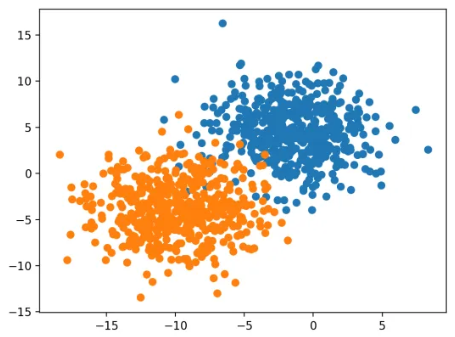
\includegraphics[width=4cm]{figures/1174017/2/binary.PNG}
		\centering
		\caption{classication}
	\end{figure}

	\item Jelaskan apa itu supervised learning dan unsupervised learning dan clustering dengan ilustrasi gambar sendiri.
	\hfill\break


	\begin{itemize}
		\item Supervised Learning
		\hfill\break
		Supervised Learning merupakan pembelajaran yang ada supervisornya. Maksudnya label di tiap data nya. Label maksudnya tag dari data yang ditambahkan dalam machine learning model. Supervised Learning mempuyai nilai input dan output yang dan mampu melakukan prediksi dan klasifikasi. Misalkan pada suatu kasus suatu provider hosting indonesia ingin melakukan ramalan tentang data pengguna website 5 bulan ke depan menggunakan analisis deret waktu. Analisis deret waktu (layaknya model regresi) menggunakan data sebelumnya untuk menggunakan peramalan. Sehingga dengan data training tersebut akan diperoleh suatu model regresi yang selanjutnya akan digunakan untuk melakukan peramalan.
		\begin{figure}[H]
		\centering
			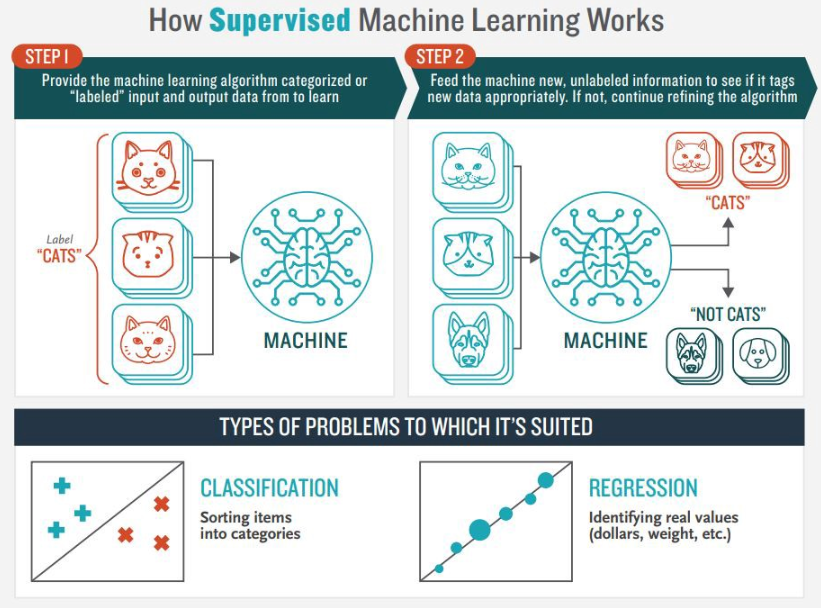
\includegraphics[width=4cm]{figures/1174017/2/supervisedlearning.PNG}
			\caption{Supervised Learning.}
		\end{figure}

		
		\item Unsupervised Learning 
		\hfill\break
		Jika unsupervised learning memiliki label sebagai dasar prediksi baik dan membuat clasification dan regression algoritma. Dalam hal lain, data real itu sangat banyak yang tidak memiliki label.Unsupervised learning tidak menggunakan label dalam memprediksi target feautures / variable. Melainkan menggunakan ke samaan dari attribut attribut yang dimiliki. Sehingga akan dilakukan kelompok kelompok (cluster). Jumlah cluster bisa unlimited.

		\begin{figure}[H]
		\centering
			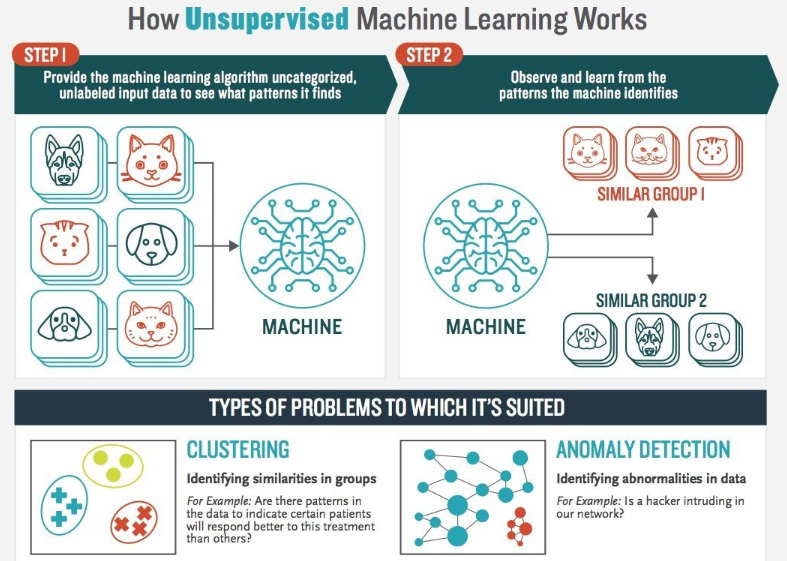
\includegraphics[width=4cm]{figures/1174017/2/unsupervisedlearning.PNG}
			\caption{Unsupervised Learning.}
		\end{figure}


		\item Clustering
		\hfill\break
		Clustering ini bertujuan untuk mengelompokan titik-titik data yang berdekatan dan mimisahkannya dengan kelompok-kelompok lain. Clustering ini dapat dilakukan secara unsupervised, artinya tidak ada contoh bagaimana seharusnya mengelompokan titik-titik tersebut.

		\begin{figure}[H]
		\centering
			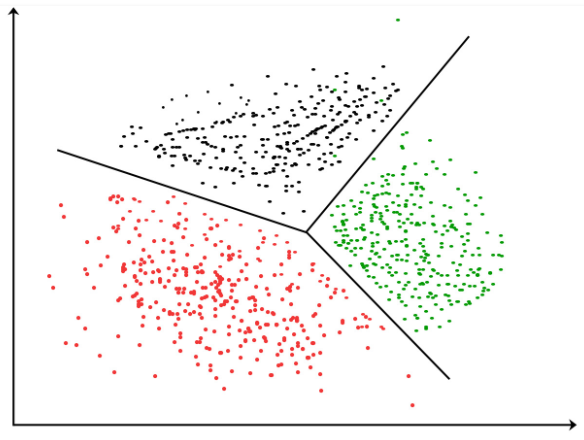
\includegraphics[width=4cm]{figures/1174017/2/clustering.PNG}
			\caption{Clustering.}
		\end{figure}
	\end{itemize}


	\item Jelaskan apa itu evaluasi dan akurasi dari buku dan disertai ilustrasi contoh dengan gambar sendiri.
	\hfill\break
	Evaluasi dan Akurasi dari buku ini merupakan suatu bentuk evaluasi yang dilaksanakan pada tahap pengembangan program dan sebelum program dimulai. Evaluasi yang dilakukan saat merencanakan suatu program. Dengan tujuan utamanya ialah untuk meyakinkan bahwa rencana akan disusun benar-benar telah sesuai dengan masalah yang ditemukan.

	\begin{figure}[H]
	\centering
		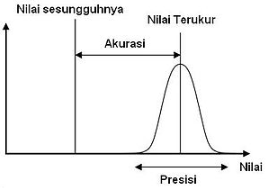
\includegraphics[width=4cm]{figures/1174017/2/akurasidanevaluasidata.PNG}
		\caption{Evaluasi dan Akurasi.}
	\end{figure}

	\item Jelaskan bagaimana cara membuat dan membaca confusion matrix, buat confusion matrix buatan sendiri.
	\hfill\break
	Confusion matrix merupakan suatu metode yang digunakan untuk melakukan perhitungan akurasi. Terdapat empat istilah diantaranya True Positive (TP), True Negative (TN), False Positive (FP) dan False Negative (FN). 
True Negative merupakan jumlah data negatif yang terdeteksi dengan benar. 
False Positive merupakan data negatif namun terdeteksi sebagai data positif. 
True Positive merupakan data positif yang terdeteksi benar. 
False Negative merupakan data positif, namun terdeteksi sebagai data negatif.

	\begin{figure}[H]
	\centering
		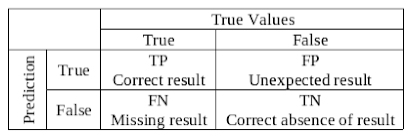
\includegraphics[width=4cm]{figures/1174017/2/confusion.PNG}
		\caption{Confusion Matrix.}
	\end{figure}

	\item Jelaskan bagaimana K-fold cross validation bekerja dengan gambar ilustrasi contoh buatan sendiri.
	\hfill\break
	Cross-validation (CV) K-Fold merupakan suatu metode statistik yang dapat digunakan untuk mengevaluasi kinerja model atau algoritma. Cross Validation K-Fold terdapat data yang dipisahkan menjadi dua subset yakni data proses pembelajaran dan data validasi. Biasanya Cross Validation K-fold digunakan karena dapat mengurangi waktu komputasi dengan tetap menjaga keakuratan estimasi.

	\begin{figure}[H]
	\centering
		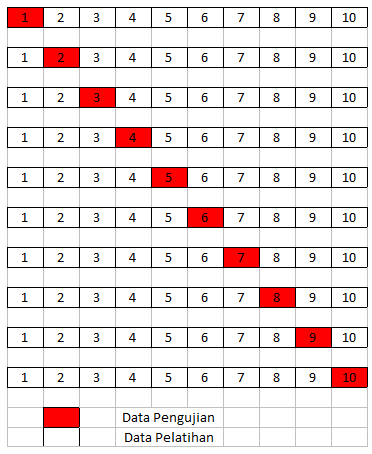
\includegraphics[width=4cm]{figures/1174017/2/k-fold.PNG}
		\caption{K-Fold Cross Validation.}
	\end{figure}

	\item Jelaskan apa itu decision tree dengan gambar ilustrasi contoh buatan sendiri.
	\hfill\break
	 Decision tree merupakan suatu metode klasifikasi untuk diinterpretasi oleh manusia berupa menggunakan metode struktur yang berbentuk seperti pohon atau struktur berhirarki.

	\begin{figure}[H]
	\centering
		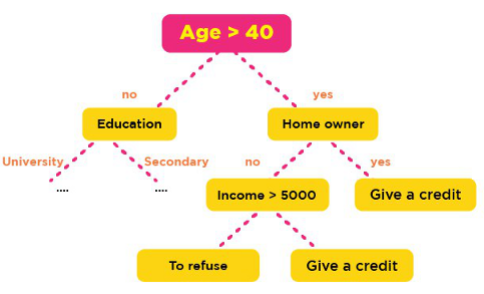
\includegraphics[width=4cm]{figures/1174017/2/decisiontree.PNG}
		\caption{Decision Tree.}
	\end{figure}

	\item Jelaskan apa itu information gain dan entropi dengan gambar ilustrasi buatan sendiri.

	\begin{itemize}
		\item Information Gain
		\hfill\break
		Information gain merupakan salah satu metode algoritma untuk menyeleksi fitur untuk menentukan batas dari kepentingan sebuah atribut. Metode information gain ini baik digunakan khususnya untuk dataset berdimensi tinggi.
Keterangan:
S = ruang (data) sample.
A = atribut.
|Si| = jumlah sample untuk nilai V.
|S| = jumlah seluruh sample data.
Entropi(Si) = sebagai sample yang memiliki nilai i

		\begin{figure}[H]
		\centering
			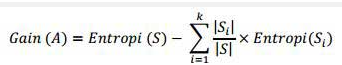
\includegraphics[width=4cm]{figures/1174017/2/informationgain.PNG}
			\caption{Information Gain.}
		\end{figure}

		\item Entropi
		\hfill\break
		Algoritma pada metode ini menggunakan konsep dari entropi. Konsep Algoritma Entropi digunakan untuk mengukur seberapa informatifnya sebuah node bisa disebut juga seberapa baiknya.

Keterangan:
S sebagai himpunan (dataset) kasus 
k sebagai banyaknya partisi S
pj sebagai probabilitas yang di dapat dari Sum(Ya) dibagi Total Kasus.
		\begin{figure}[H]
		\centering
			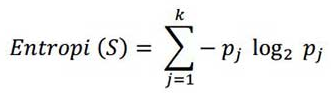
\includegraphics[width=4cm]{figures/1174017/2/entropi.PNG}
			\caption{Entropi.}
		\end{figure}
	\end{itemize}
\end{enumerate}


\subsection{Praktek}
\begin{enumerate}
	\item Soal 1
	\hfill\break
	\lstinputlisting[firstline=10, lastline=13]{src/1174017/2/1174017.py}
	Kode di atas digunakan untuk mengimpor atau mengirim library pandas sebagai pd. Kemudian ditentukan variabel "lampung" untuk dipanggil dataset diperoleh dari data student-mat.csv. Hasilnya adalah sebagai berikut :
	\begin{figure}[H]
	\centering
		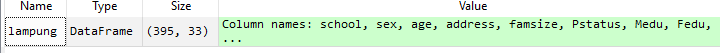
\includegraphics[width=4cm]{figures/1174017/2/hasilsoal1.PNG}
		\caption{Hasil Soal 1.}
	\end{figure}

	\item Soal 2
	\hfill\break
	\lstinputlisting[firstline=18, lastline=21]{src/1174017/2/1174017.py}
	Kode di atas ada bagian mendeklarasikan pass/fail nya data berdasarkan G1+G2+G3. Dengan ketentuan nilai pass nya yaitu sama dengan 30. kemudian pada variabel lampung dideklarasikan jika baris dengan G1+G2+G3 ditambahkan, dan hasilnya sama dengan 35 maka axisnya 1. Hasilnya adalah sebagai berikut :
	\begin{figure}[H]
	\centering
		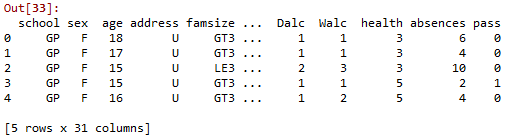
\includegraphics[width=4cm]{figures/1174017/2/hasilsoal2.PNG}
		\caption{Hasil Soal 2.}
	\end{figure}
	
	\item Soal 3
	\hfill\break
	\lstinputlisting[firstline=26, lastline=30]{src/1174017/2/1174017.py}
	One-hot encoding adalah proses di mana variabel kategorikal dikonversi menjadi bentuk yang dapat disediakan untuk algoritma ML untuk melakukan pekerjaan yang lebih baik dalam prediksi. Metode head ini digunakan untuk mengembalikan baris n atas 5 secara default dari frame atau seri data Karena saya memuat data menggunakan. Hasilnya adalah sebagai berikut :
	\begin{figure}[H]
	\centering
		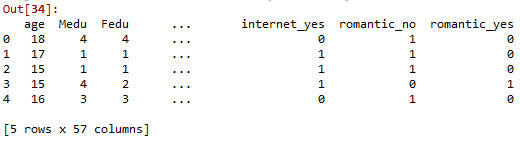
\includegraphics[width=4cm]{figures/1174017/2/hasilsoal3.PNG}
		\caption{Hasil Soal 3.}
	\end{figure}

	\item Soal 4
	\hfill\break
	\lstinputlisting[firstline=35, lastline=52]{src/1174017/2/1174017.py}
	Sammple digunakan untuk mengembalikan sampel acak item dari objek. Pada bagian tersebut, terdapat train dan test yaing digunakan untuk untuk membagi train, test dan kemudian membagi lagi train ke validasi dan test. Kemudia akan mengimport module numpy sebagai np yang akan digunakan untuk mengembalikan nilai passing dari pelajar dari keseluruhan dataset dengan cara print. Hasilnya adalah sebagai berikut :
	\begin{figure}[H]
	\centering
		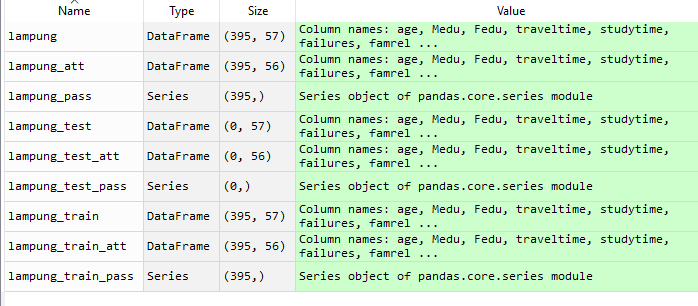
\includegraphics[width=4cm]{figures/1174017/2/hasilsoal4.PNG}
		\caption{Hasil Soal 4.}
	\end{figure}

	\item Soal 5
	\hfill\break
	\lstinputlisting[firstline=57, lastline=60]{src/1174017/2/1174017.py}
	Dari librari scikitlearn import modul tree. Kemudian definisikan variabel kibang dengan menggunakan DecisionClassifier. Kemudian pada variabel kibang terdapat Criterion yaitu suatu fungsi untuk mengukur kualitas split, setelah itu agar DecisionTreeClassifier dapat dijalankan gunakan perintah fit. Hasilnya adalah sebagai berikut :
	\begin{figure}[H]
	\centering
		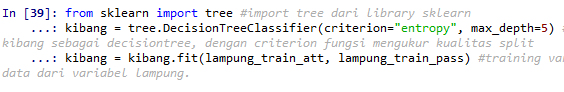
\includegraphics[width=4cm]{figures/1174017/2/hasilsoal5.PNG}
		\caption{Hasil Soal 5.}
	\end{figure}

	\item Soal 6
	\hfill\break
	\lstinputlisting[firstline=65, lastline=71]{src/1174017/2/1174017.py}
	Graphviz adalah perangkat lunak visualisasi grafik open source. Visualisasi grafik adalah cara mewakili informasi struktural sebagai diagram grafik dan jaringan abstrak. Hasilnya adalah sebagai berikut :
	\begin{figure}[H]
	\centering
		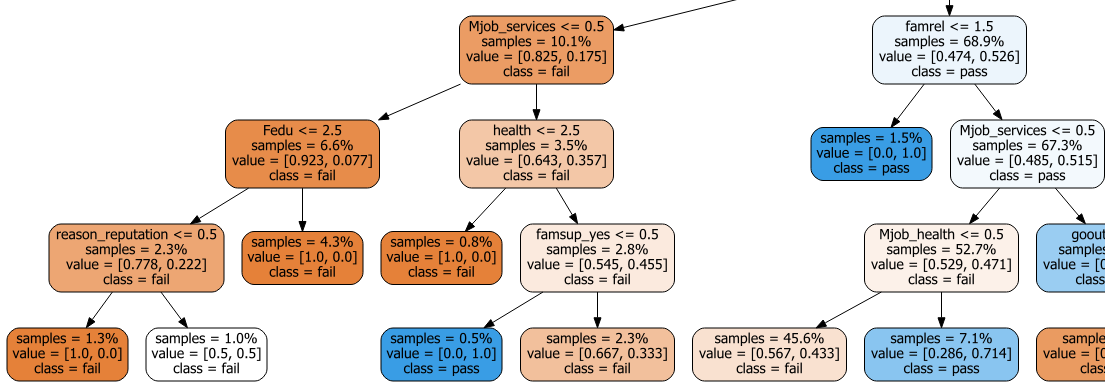
\includegraphics[width=4cm]{figures/1174017/2/hasilsoal6.PNG}
		\caption{Hasil Soal 6.}
	\end{figure}

	\item Soal 7
	\hfill\break
	\lstinputlisting[firstline=76, lastline=79]{src/1174017/2/1174017.py}
	Tree.export graphviz merupakan fungsi yang menghasilkan representasi Graphviz dari decision tree, yang kemudian ditulis ke outfile.Disini akan menyimpan classifiernya, akan meng ekspor file student performance jika salah akan mengembalikan nilai fail. Hasilnya adalah sebagai berikut :
	\begin{figure}[H]
	\centering
		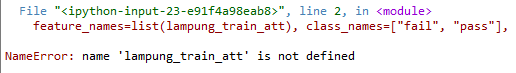
\includegraphics[width=4cm]{figures/1174017/2/hasilsoal7.PNG}
		\caption{Hasil Soal 7.}
	\end{figure}

	\item Soal 8
	\hfill\break
	\lstinputlisting[firstline=84, lastline=86]{src/1174017/2/1174017.py}
	Score juga disebut prediksi, dan merupakan proses menghasilkan nilai berdasarkan model pembelajaran mesin yang terlatih, diberi beberapa data input baru. Nilai atau skor yang dibuat dapat mewakili prediksi nilai masa depan, tetapi mereka juga mungkin mewakili kategori atau hasil yang mungkin. Jadi disini kibang akan memprediksi nilai dari lampung test att dan test pass Hasilnya adalah sebagai berikut :
	\begin{figure}[H]
	\centering
		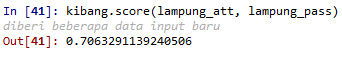
\includegraphics[width=4cm]{figures/1174017/2/hasilsoal8.PNG}
		\caption{Hasil Soal 8.}
	\end{figure}

	\item Soal 9
	\hfill\break
	\lstinputlisting[firstline=91, lastline=94]{src/1174017/2/1174017.py}
	Skrip ini akan mengevaluasi score dengan validasi silang. Dimana variabel scores berisikan crossvalscore yang merupakan fungsi pembantu pada estimator dan dataset. Kemudian akan menampilkan score rata rata dan kurang lebih dua standar deviasi yang mencakup 95 persen score. Hasilnya adalah sebagai berikut :
	\begin{figure}[H]
	\centering
		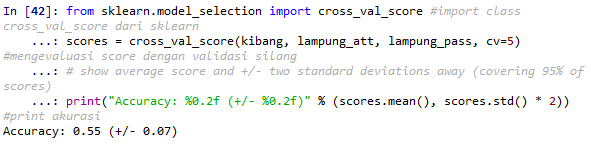
\includegraphics[width=4cm]{figures/1174017/2/hasilsoal9.PNG}
		\caption{Hasil Soal 9.}
	\end{figure}

	\item Soal 10
	\hfill\break
	\lstinputlisting[firstline=99, lastline=104]{src/1174017/2/1174017.py}
	Pada skrip ini menunjukkan seberapa dalam tree itu. Semakin dalam tree, semakin banyak perpecahan yang dimilikinya dan menangkap lebih banyak informasi tentang data. variabel kibang akan mendefinisikan tree nya yang kemudian variabel scores akan mengevaluasi score dengan validasi silang. disini mendefinisikan decision tree dengan kedalaman mulai dari 1 hingga 20. Hasilnya adalah sebagai berikut :
	\begin{figure}[H]
	\centering
		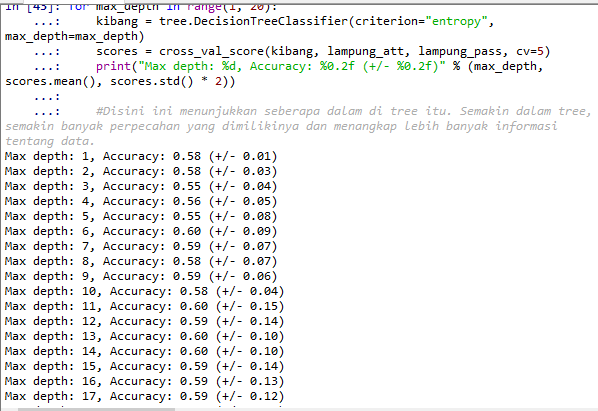
\includegraphics[width=4cm]{figures/1174017/2/hasilsoal10.PNG}
		\caption{Hasil Soal 10.}
	\end{figure}

	\item Soal 11
	\hfill\break
	\lstinputlisting[firstline=109, lastline=119]{src/1174017/2/1174017.py}
	Depth acc akan membuat array kosong dengan mengembalikan array baru dengan bentuk dan tipe yang diberikan, tanpa menginisialisasi entri. Dengan 19 sebagai bentuk array kosong, 3 sebagai output data-type dan float urutan kolomutama (gaya Fortran) dalam memori. variabel kibang yang akan melakukan split score akan mengvalidasi score secara silang. Hasilnya adalah sebagai berikut :
	\begin{figure}[H]
	\centering
		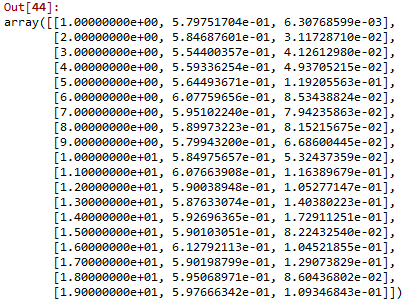
\includegraphics[width=4cm]{figures/1174017/2/hasilsoal11.PNG}
		\caption{Hasil Soal 11.}
	\end{figure}

	\item Soal 12
	\hfill\break
	\lstinputlisting[firstline=124, lastline=127]{src/1174017/2/1174017.py}
	Mengimpor librari dari matplotlib yaitu pylot sebagai plt fig dan ax menggunakan subplots untuk membuat gambar dan satu set subplot. axerrorbar akan membuat error bar kemudian grafik akan ditampilkan menggunakan show. Hasilnya adalah sebagai berikut :
	\begin{figure}[H]
	\centering
		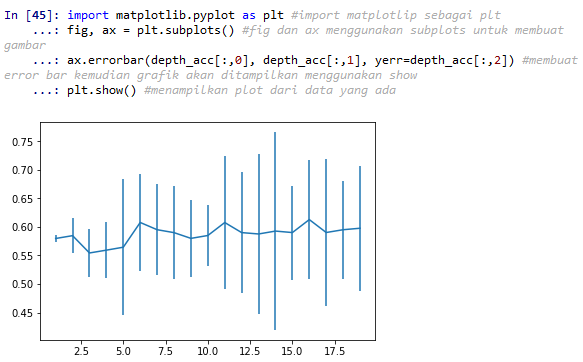
\includegraphics[width=4cm]{figures/1174017/2/hasilsoal12.PNG}
		\caption{Hasil Soal 12.}
	\end{figure}
\end{enumerate}


\subsection{Penanganan Error}
\begin{enumerate}
	\item ScreenShoot Error
	\begin{figure}[H]
		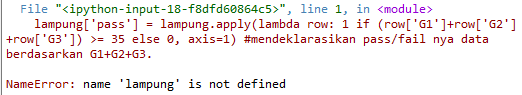
\includegraphics[width=4cm]{figures/1174017/2/errorname.PNG}
		\centering
		\caption{NameError}
	\end{figure}
	\begin{figure}[H]
		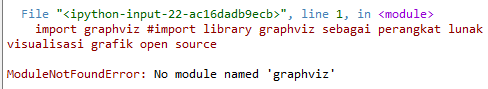
\includegraphics[width=4cm]{figures/1174017/2/notmoduleerror.PNG}
		\centering
		\caption{ModuleNotFoundError}
	\end{figure}
	\begin{figure}[H]
		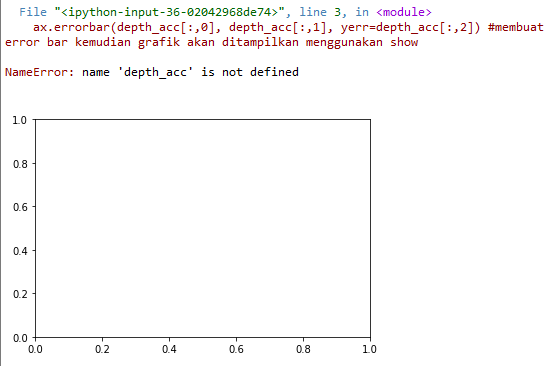
\includegraphics[width=4cm]{figures/1174017/2/errorimportmatplotlib.PNG}
		\centering
		\caption{ErrorImportMatplotlib}
	\end{figure}
	\item Tuliskan Kode Error dan Jenis Error
	\begin{itemize}
		\item NameError
		\item ModuleNotFoundError
		\item ErrorImportMatplotlib
	\end{itemize}

	\item Cara Penangan Error
	\begin{itemize}
		\item NameError
		\hfill\break
		Error terdapat pada penamaan alias pd yang tidak terdefenisikan, seharusnya jika variabel lampung, maka hasilnya lampung juga.
		\item ModuleNotFoundError
		\hfill\break
		Error terdapat pada kesalahan modul graphviz yang belum di install, solusinya ialah menginstall library tersebut di anaconda.
		\item ErrorImportMatplotlib
		\hfill\break
		ErrorImportMatplotlib harus ada import dari matplotlib terlebih dahulu.
	\end{itemize}
\end{enumerate}

\subsection{Bukti Tidak Plagiat}
\begin{figure}[H]
\centering
	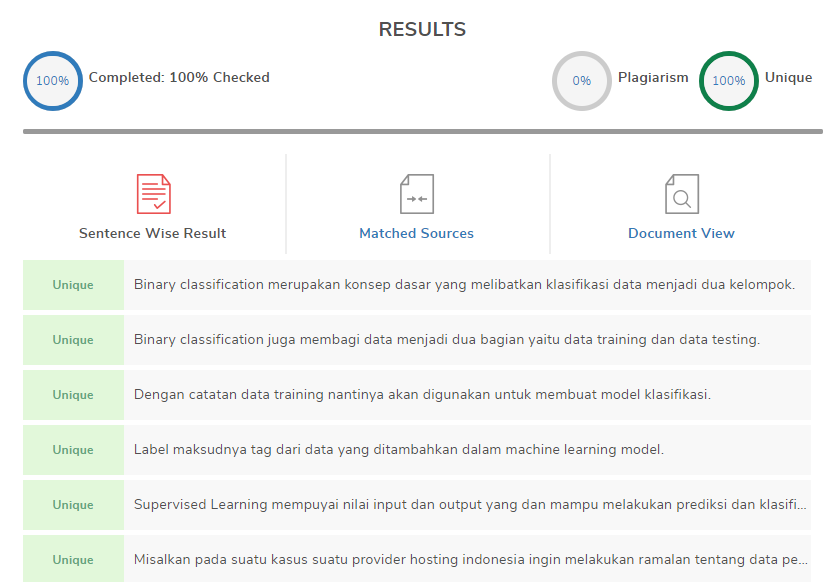
\includegraphics[width=4cm]{figures/1174017/2/bukanplagiat.PNG}
	\caption{Bukti Tidak Melakukan Plagiat Chapter 2}
\end{figure}